\begin{section}{Resultados}
	El siguiente gráfico se realizó para ajustar un parámetro ($epsilon$) del programa que sirve para generar las matrices mal condicionadas. Recordar que una matriz mal condicionada se construye a partir de un vector que resulta en las filas de la misma y luego se le suma el $epsilon$a los elementos de la diagonal para que quede inversible.
	
	Con esta prueba esperamos ver que cuanto menor es el $epsilon$ mayor es el número de condición de la matriz debido a que las filas están más cerca de ser linealmente dependientes y por ende la matriz más cerca de ser singular.

	El gráfico muestra el número de condición de la matriz en función de su dimensión para los siguientes valores de $epsilon$: $1$, $1e^{-1}$, $1e^{-2}$, $1e^{-3}$, $1e^{-4}$, $1e^{-5}$ y $1e^{-6}$. Elegimos esos valores de $epsilon$ ya que para generarlos tenemos una variable $v$ ($unsigned\;int$) que itera por los múltiplos de $10$ (empezando en $1$), siendo $epsilon$ igual a $1.0/v$. El mayor múltiplo de $10$ que $v$ es capaz de almacenar es $1e^9$ pero con $epsilon$ igual a $1e^{-7}$, $1e^{-8}$ y $1e^{-9}$ las matrices generadas quedaban singulares en muchas ocasiones, suponemos que eso se debe a que estos valores de $epsilon$ ya son despreciables ($cero$) y al sumarle ese valor a la diagonal no conseguimos filas linealmente dependientes como queremos.
	
	Corrimos las pruebas para matrices de dimensión $2$ a dimensión $50$.
	El eje que corresponde al \texttt{número de condición} está en escala logarítmica para poder apreciar mejor los valores correspondientes dado que estos crecen exponencialmente.

	\begin{figure}[H]
	  \centering
		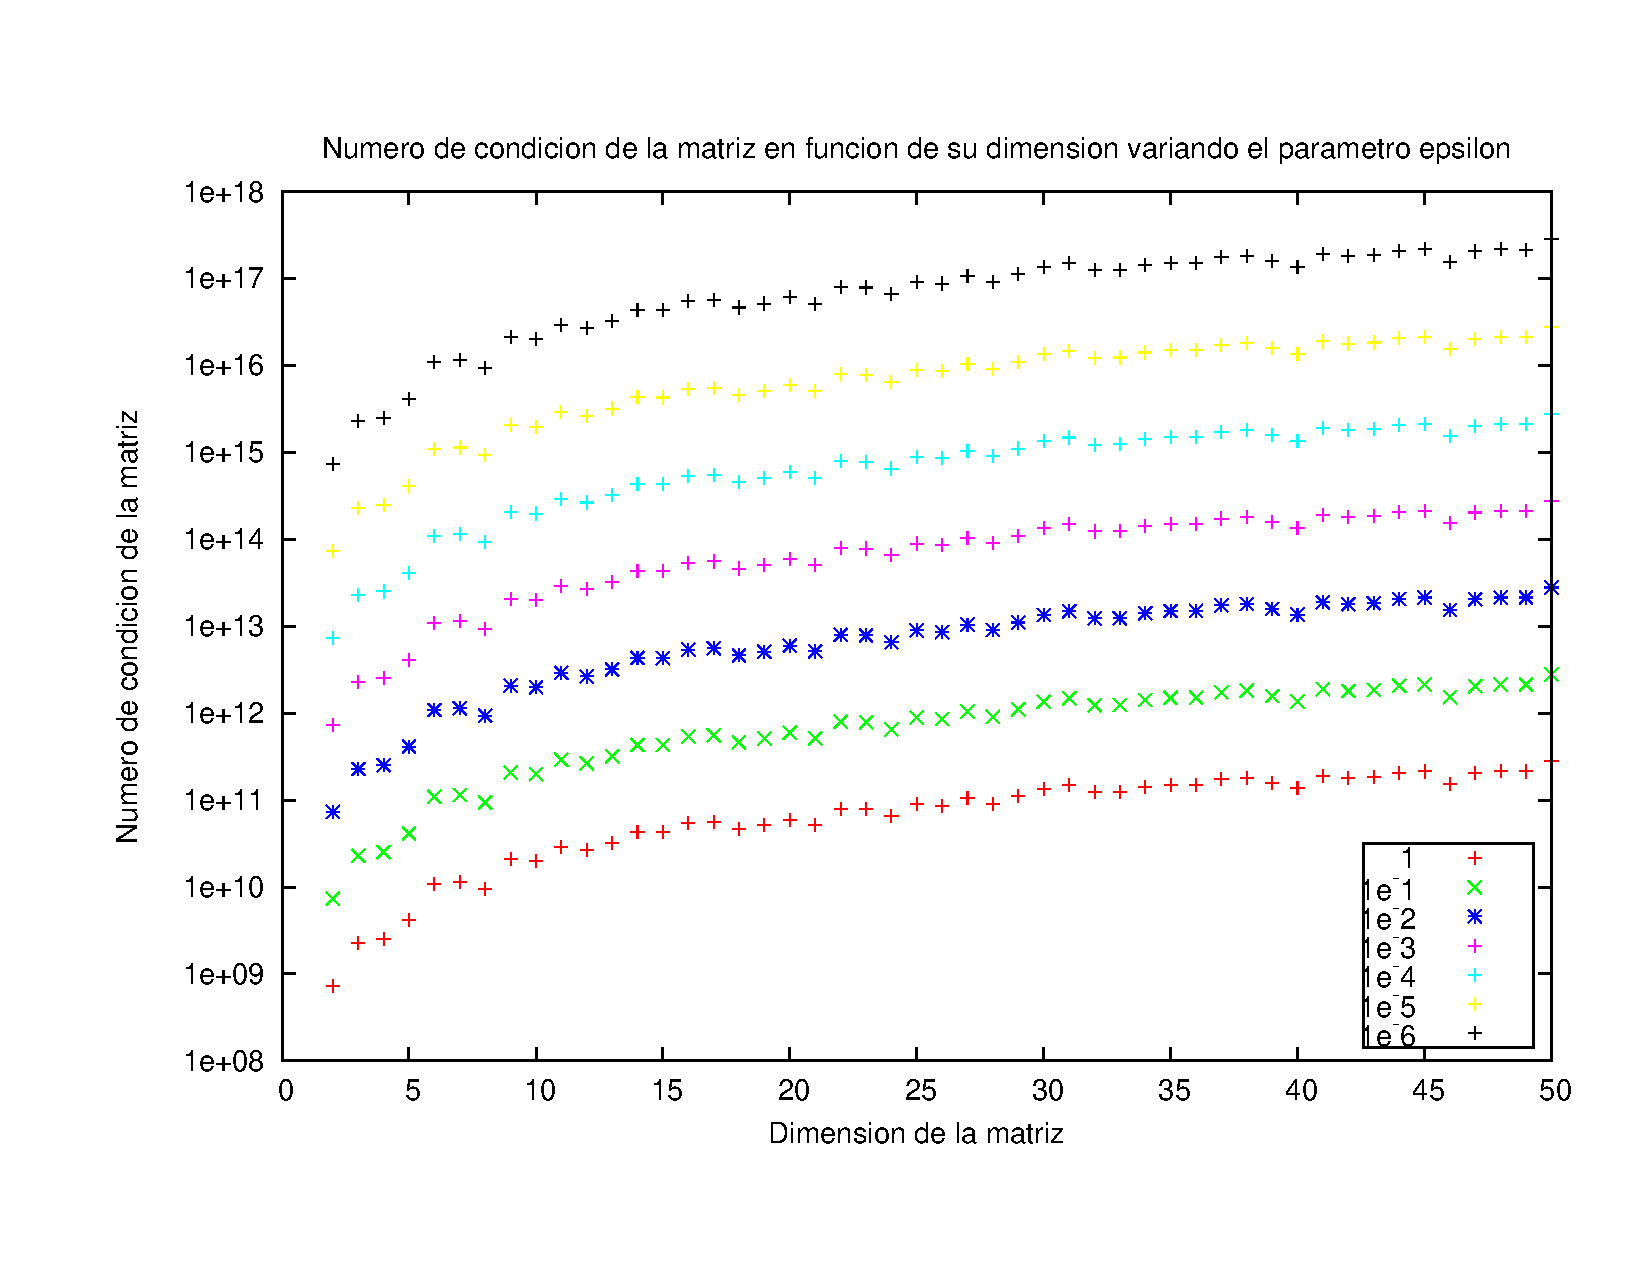
\includegraphics[width=14cm]{graficos/ajuste_epsilon.pdf}
	  \caption{Número de condición de la matriz en función de su dimensión variando el parámetro epsilon}
	  \label{fig:epsilon}
	\end{figure}
	
	\VSP
	
	Para comparar los métodos de resolución de sistemas de ecuaciones lineales implentados (inversa y LU) realizamos el siguiente gráfico que muestra la exactitud de la solución en función de la dimensión de la matriz. Corrimos las pruebas para matrices de dimensión $2$ a dimensión $50$.
	
	Para medir la exactitud de la solución tomamos la norma2 de la diferencia entre la solución calculada y la solución real.
	
	El gráfico se presenta bajo una escala logaritmica en el eje $y$.
	
	\begin{figure}[H]
	  \centering
		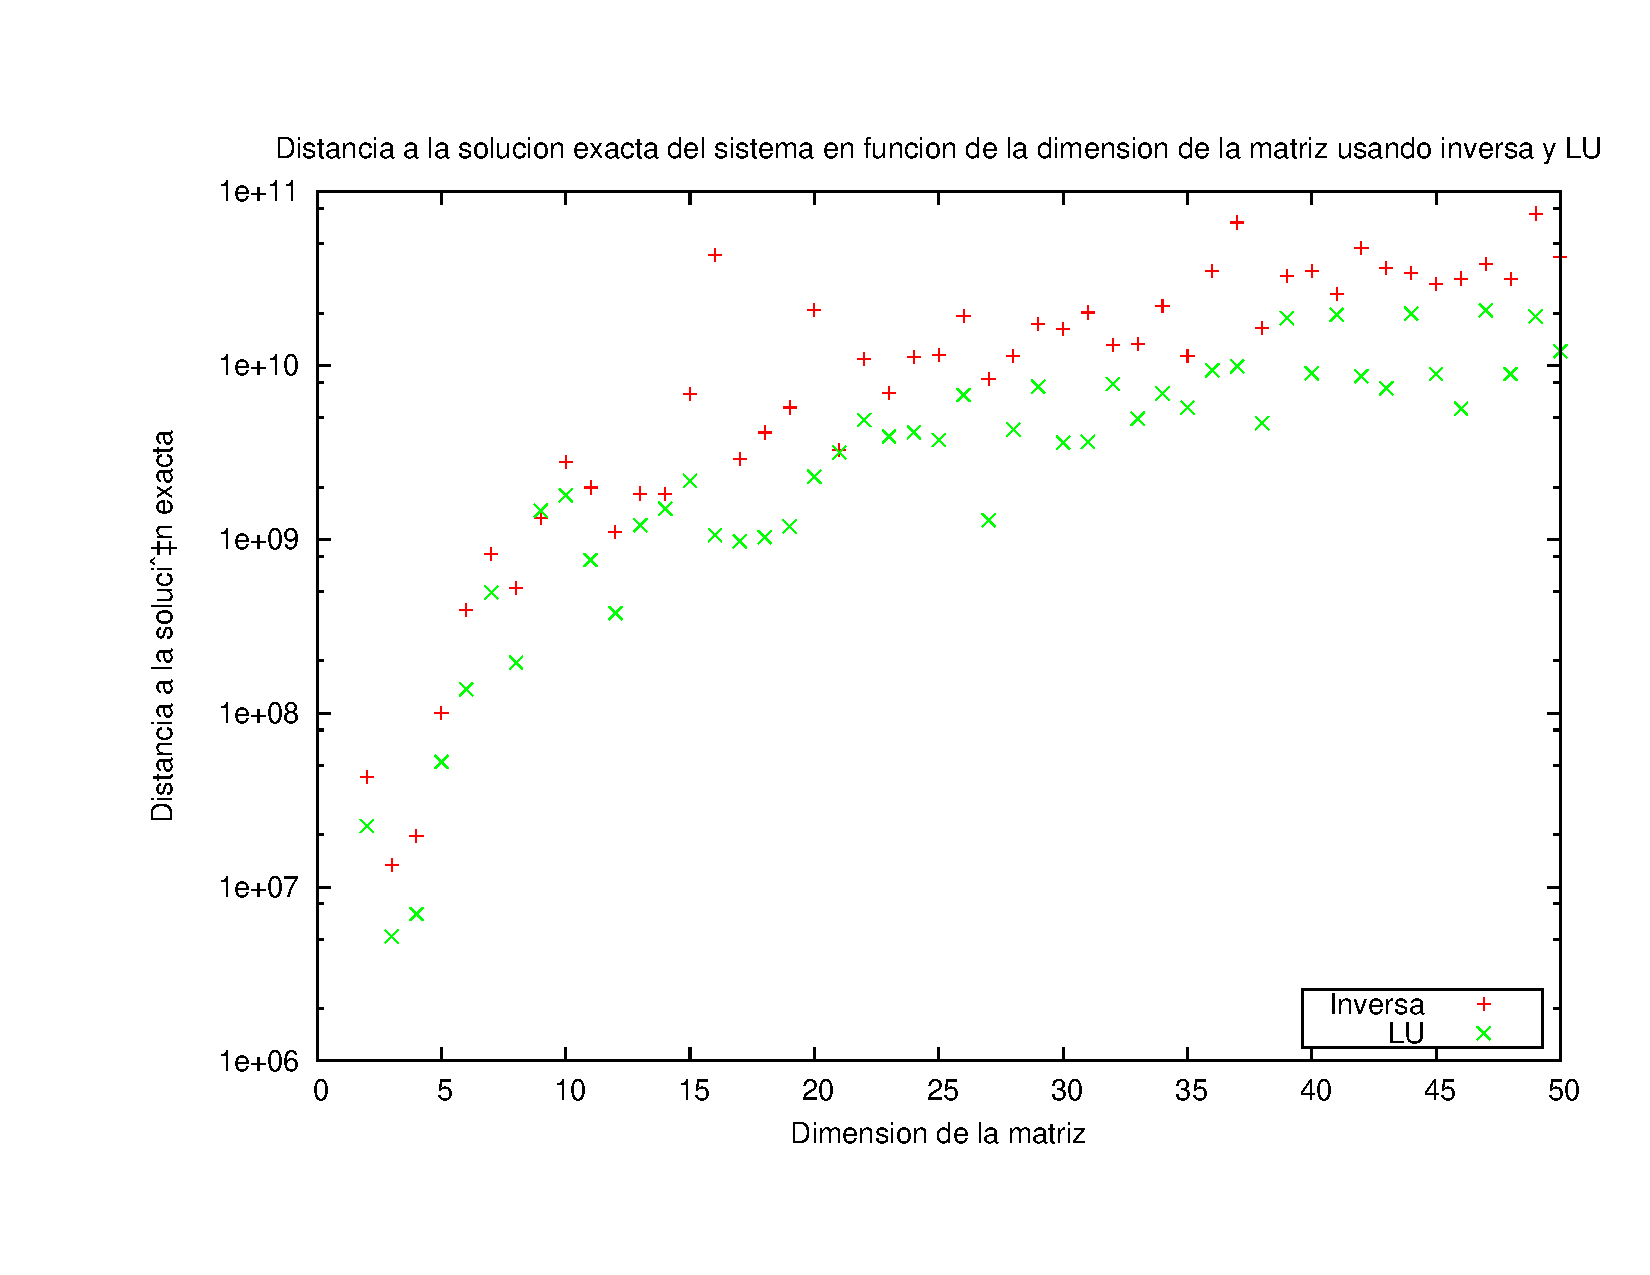
\includegraphics[width=14cm]{graficos/inv_vs_lu.pdf}
	  \caption{Distancia a la solución exacta del sistena en funcion de la dimension de la matriz usando el método de la inversa y factorizacion LU}
	  \label{fig:inv_vs_lu}
	\end{figure}
	
	\VSP
	
	%El gráfico anterior representa una corrida del test el cual genera una instancia ($A$, $x$ y $d$) para cada dimensión y resuelve el sistema $Ax=d$ usando los distintos métodos. Para generar la matriz y los vectores se usan coeficientes aleatorios por lo que los resultados provistos por esta prueba se pueden ver afectados por las instancias elegidas.
	
	Realizamos el siguiente gráfico para comprobar que la aproximación a la posición enemiga mejora al tomar el promedio entre todas las posiciones calculadas hasta el momento. Esperamos mediante esta prueba dar sustento a nuestra estrategia.
	
	El gráfico muestra la exactitud del ataque (norma2 de la diferencia entre donde impacta el proyectil y donde realmente está el enemigo) en función de la cantidad de turnos trascurridos para un disparo directo y un disparo tomando promedio de las posiciones calculadas previamente.
	Se utilizó LU para encontrar la posición del enemigo dada la información del turno anterior (Ver justificación en sección \texttt{Discusión}).
	
	Corrimos las pruebas para matrices de dimensión $5$ y de dimensión $20$ (elegimos esas dimensiones arbitrariamente, lo unico que buscamos es que esten el rango de lo que se va a usar y que no sean muy cercanas entre sí) hasta el turno $500$ (consideramos una cantidad de turnos sufieciente para ver lo que esperamos). El eje $y$ está en escala logarítmica.
	
	
	\begin{figure}[H]
	  \centering
		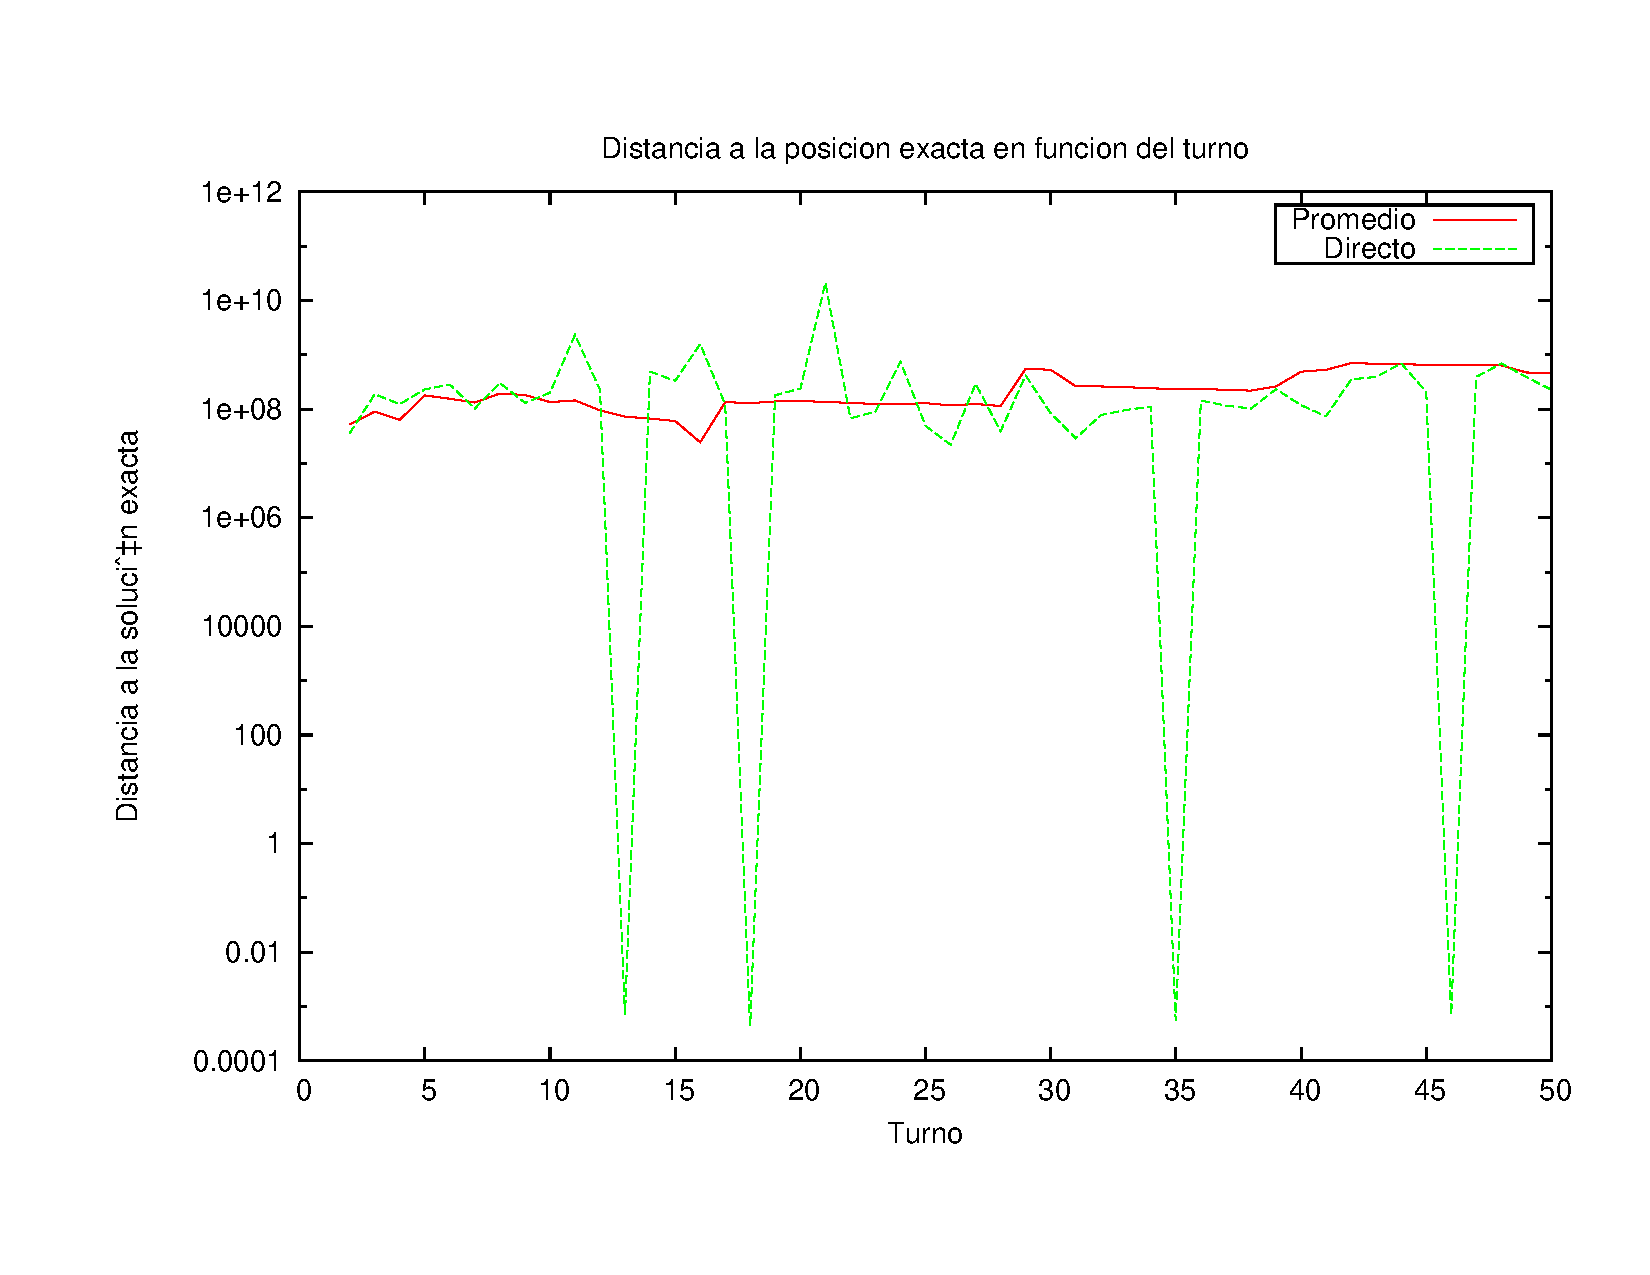
\includegraphics[width=14cm]{graficos/prom_vs_direct.pdf}
	  \caption{Distancia a la posición exacta en funcion del turno usando promedio de las posiciones calculadas anteriormente y disparando directamente}
	  \label{fig:prom_vs_direct}
	\end{figure}
	
	\VSP
\end{section}
